\documentclass{article}
\usepackage{mathptmx}
\usepackage{url,latexsym,amsmath,amsthm,xspace,rotating,multirow,multicol,xspace,amssymb,paralist}
\usepackage{euscript}
\usepackage{fancybox,xcolor}
\usepackage{longtable}
\usepackage{paralist}
\usepackage[normalem]{ulem}
\usepackage[pdftex]{hyperref}

\usepackage{url}
\usepackage{latexsym}

\usepackage{times}
\usepackage{amsmath}
\usepackage{amsthm}
\usepackage{amssymb}
\usepackage{graphicx}
\usepackage{xspace}
\usepackage{tabularx}
\usepackage{multicol}
\usepackage{multirow}
%\usepackage{hyperref}
\usepackage{url}
%\usepackage{natbib}
\usepackage{wrapfig}
\usepackage{comment}
\usepackage{listings}
\usepackage{color}
\usepackage[utf8]{inputenc}
\usepackage{fancyvrb}
\usepackage{booktabs}
\usepackage{color}
\usepackage[normalem]{ulem}

\newcommand{\obs}{\text{obs}}
\newcommand{\mis}{\text{mis}}

\newcommand{\qt}[1]{\left<#1\right>}
\newcommand{\ql}[1]{\left[#1\right]}
\newcommand{\hess}{\mathbf{H}}
\newcommand{\jacob}{\mathbf{J}}
\newcommand{\hl}{HL}
\newcommand{\cost}{\mathcal{L}}
\newcommand{\lout}{\mathbf{r}}
\newcommand{\louti}{r}
\newcommand{\outi}{y}
\newcommand{\out}{\mathbf{y}}
\newcommand{\gauss}{\mathbf{G_N}}
\newcommand{\eye}{\mathbf{I}}
\newcommand{\softmax}{\phi}
\newcommand{\targ}{\mathbf{t}}
\newcommand{\metric}{\mathbf{G}}
\newcommand{\sample}{\mathbf{z}}
\newcommand{\f}{\text{f}}
%\newcommand{\log}{\text{log}}

\newcommand{\bmx}[0]{\begin{bmatrix}}
\newcommand{\emx}[0]{\end{bmatrix}}
\newcommand{\qexp}[1]{\left<#1\right>}
\newcommand{\vect}[1]{\mathbf{#1}}
\newcommand{\vects}[1]{\boldsymbol{#1}}
\newcommand{\matr}[1]{\mathbf{#1}}
\newcommand{\var}[0]{\operatorname{Var}}
\newcommand{\std}[0]{\operatorname{std}}
\newcommand{\cov}[0]{\operatorname{Cov}}
\newcommand{\diag}[0]{\operatorname{diag}}
\newcommand{\matrs}[1]{\boldsymbol{#1}}
\newcommand{\va}[0]{\vect{a}}
\newcommand{\vb}[0]{\vect{b}}
\newcommand{\vc}[0]{\vect{c}}
\newcommand{\ve}[0]{\vect{e}}

\newcommand{\vh}[0]{\vect{h}}
\newcommand{\vv}[0]{\vect{v}}
\newcommand{\vx}[0]{\vect{x}}
\newcommand{\vz}[0]{\vect{z}}
\newcommand{\vw}[0]{\vect{w}}
\newcommand{\vs}[0]{\vect{s}}
\newcommand{\vf}[0]{\vect{f}}
\newcommand{\vi}[0]{\vect{i}}
\newcommand{\vo}[0]{\vect{o}}
\newcommand{\vy}[0]{\vect{y}}
\newcommand{\vg}[0]{\vect{g}}
\newcommand{\vm}[0]{\vect{m}}
\newcommand{\vu}[0]{\vect{u}}
\newcommand{\vL}[0]{\vect{L}}
\newcommand{\vr}[0]{\vect{r}}
\newcommand{\vone}[0]{\vect{1}}
\newcommand{\mW}[0]{\matr{W}}

\newcommand{\mE}[0]{\matr{E}}
\newcommand{\mG}[0]{\matr{G}}
\newcommand{\mX}[0]{\matr{X}}
\newcommand{\mY}[0]{\matr{Y}}
\newcommand{\mQ}[0]{\matr{Q}}
\newcommand{\mU}[0]{\matr{U}}
\newcommand{\mF}[0]{\matr{F}}
\newcommand{\mV}[0]{\matr{V}}
\newcommand{\mA}{\matr{A}}
\newcommand{\mC}{\matr{C}}
\newcommand{\mD}{\matr{D}}
\newcommand{\mS}{\matr{S}}
\newcommand{\mI}{\matr{I}}
\newcommand{\td}[0]{\text{d}}
\newcommand{\TT}[0]{\vects{\theta}}
\newcommand{\vsig}[0]{\vects{\sigma}}
\newcommand{\valpha}[0]{\vects{\alpha}}
\newcommand{\vmu}[0]{\vects{\mu}}
\newcommand{\vzero}[0]{\vect{0}}
\newcommand{\tf}[0]{\text{m}}
\newcommand{\tdf}[0]{\text{dm}}
\newcommand{\grad}[0]{\nabla}
\newcommand{\alert}[1]{\textcolor{red}{#1}}
\newcommand{\N}[0]{\mathcal{N}}
\newcommand{\BB}[0]{\mathcal{B}}
\newcommand{\LL}[0]{\mathcal{L}}
\newcommand{\HH}[0]{\mathcal{H}}
\newcommand{\RR}[0]{\mathbb{R}}
\newcommand{\MM}[0]{\mathcal{M}}
\newcommand{\OO}[0]{\mathbb{O}}
\newcommand{\II}[0]{\mathbb{I}}
\newcommand{\Scal}[0]{\mathcal{S}}
\newcommand{\sigmoid}{\sigma}
\newcommand{\E}[0]{\mathbb{E}}
\newcommand{\enabla}[0]{\ensuremath{%
    \overset{\raisebox{-0.3ex}[0.5ex][0ex]{%
    \ensuremath{\scriptscriptstyle e}}}{\nabla}}}
\newcommand{\enhnabla}[0]{\nabla_{\hspace{-0.5mm}e}\,}


\newcommand{\todo}[1]{{\Large\textcolor{red}{#1}}}
\newcommand{\done}[1]{{\Large\textcolor{green}{#1}}}
\newcommand{\dd}[1]{\ensuremath{\mbox{d}#1}}

\DeclareMathOperator*{\argmax}{\arg \max}
\DeclareMathOperator*{\argmin}{\arg \min}
\newcommand{\newln}{\\&\quad\quad{}}

\newcommand{\KL}{\text{KL}}
\newcommand{\data}{\text{data}}
\newcommand{\rect}{\text{rect}}
\newcommand{\maxout}{\text{maxout}}
\newcommand{\train}{\text{train}}
\newcommand{\val}{\text{val}}
\newcommand{\test}{\text{test}}
\newcommand{\Ax}{\mathcal{A}_x}
\newcommand{\Ay}{\mathcal{A}_y}
\newcommand{\ola}{\overleftarrow}
\newcommand{\ora}{\overrightarrow}
\newcommand{\ov}{\overline}
\newcommand{\ts}{\rule{0pt}{2.6ex}}       % Top strut
\newcommand{\ms}{\rule{0pt}{0ex}}         % Middle strut
\newcommand{\bs}{\rule[-1.2ex]{0pt}{0pt}} % Bottom strut
\newcommand{\specialcell}[2][c]{%
  \begin{tabular}[#1]{@{}c@{}}#2\end{tabular}}


%\usepackage{bibentry}
%\nobibliography*

\begin{document}

\title{DS-GA 3001: Natural Language Understanding with Distributed Representation}
\author{Kyunghyun Cho\\New York University}

\maketitle
\pagenumbering{arabic}

{\it 
    Note that this lecture note is and will be constantly updated throughout
    the semester. Please, check for the latest version frequently.
}


\section{Introduction}

This lecture is going to be the only one where I discuss some philosophical,
meaning nonpractical, arguments, because accoring to Chris Manning and Hinrich
Schuetze, ``{\it even practically-minded people have to confront the issue of
what prior knowledge to try to build into their model}''
\cite{manning1999foundations}. 

\subsection{Route we will {\it not} take}

\subsubsection{What is Language?}

The very first question we must ask ourselves before starting this course is the
question of what natural language is. Of course, the rest of this course does
not in any way require us to know what natural language is, but it is a
philosophical question I recommend everyone, including myself, to ponder upon
once a while. 

When I start talking about languages with anyone, there is a single person who
never misses to be mentioned, that is Noam Chomsky. His view has greatly
influenced the modern linguistics, and although many linguists I have talked to
claim that their work and field have long moved on from Chomsky's, I can feel
his shadow all over them. 

My first encounter with Chomsky was at the classroom of $<$Automata$>$ from my
early undergrad years. I was not the most attentive student back then, and all I
can remember is Chomsky's hierarchy and how it has shaped our view on languages,
in this context, programming/computer languages.  A large part of the course was
dedicated to explaining which class of languages emerges given a set of
constraints on a set of {\it generating rules}, or production rules. 

For instance, if we are given a set of generating rules that do not depend on
the context/meaning of non-terminal symbols (context-free grammar, CFG), we get
a context-free language. If we put a bit of constraints to CFG that each
generating rule is such that a non-terminal symbol is replaced by either a
terminal symbol, a terminal symbol by a non-terminal symbol or an empty symbol,
then we get a regular grammar. Similarly to CFG, we get a regular language from
the regular grammar, and the regular language is a subset of the context-free
language.

What Chomsky believes is that this kind of approach applies also to human
languages, or natural languages. There exists a set of generating rules that
{\it generates} a natural language. But, then, the obvious question to follow is
where those generating rules are. Where are they stored? How are they stored? Do
we have separate generating rules for different languages? 

\subsubsection{Language Understanding}

\paragraph{Understanding Human Language}

Those questions are interesting, but out of scope for this course. Those
questions are the ones linguists try to answer. Generative linguistics aims at
figuring out what those rules are, how they are combined to form a valid
sentence, how they are adapted to different languages and so on. We will leave
these to linguists and continue on to our journey of {\it building a machine
that understands human languages}. 

\paragraph{Natural Language Understanding}

So, let's put these questions aside and trust Chomsky that we, humans, are
specially designed to store those generating rules somewhere in the brain
\cite{chomsky1959review,carnie2013syntax}. Or, better yet, let's trust Chomsky
that there's a universal grammar {\it built in} our brain. In other words, let's
say we were born with this set of generating rules for natural languages, and
while growing, we have adapted this universal grammar toward our native tongue
(language variation).

When we decide to speak of something (whatever that is and however implausible
that is), our brain quickly picks up a sequence of some of those generating
rules and starts generating a sentence accordingly. Of course, those rules do
not generate a sentence directly, but generates a sequence of control signals to
move our muscles to make sound. When heard by other people who understand your
language, the sound becomes a sentence.

In our case, we are more interested in a {\it machine} hearing that sound, or a
sentence from here on. When a machine heard this sentence, what would/should a
{\it language understanding machine} do to understand a language, or more simply
a sentence? Again, we are assuming that this sentence was generated from
applying a sequence of the existing generating rules. 

Under our assumption, a natural first step that comes to my mind is to figure
out that sequence of the generating rules which led to the sentence. Once the
sequence is found, or in a fancier term, inferred, the next step will be to
figure out what kind of mental state of the speaker led to those generating
rules. 

Let's take an example sentence ``{\it Our company is training workers}'' (from
Sec. 1.3 of \cite{manning1999foundations}), which is a horrible choice, because
this was used as an example of ambiguity in parsing. Regardless, a speaker
obviously has an awesome image of her company which trains its workers and wants
to tell a machine about this. This mental state is used to select the following
generating rules (assuming a phrase structure grammar)\footnote{
    Stanford Parser: \url{http://nlp.stanford.edu:8080/parser}
}:
\begin{verbatim}
    (ROOT
      (S
          (NP (PRP$ Our) (NN company))
              (VP (VBZ is)
                    (VP (VBG training)
                            (NP (NNS workers))))))
\end{verbatim}

\begin{figure}[ht]
    \centering
    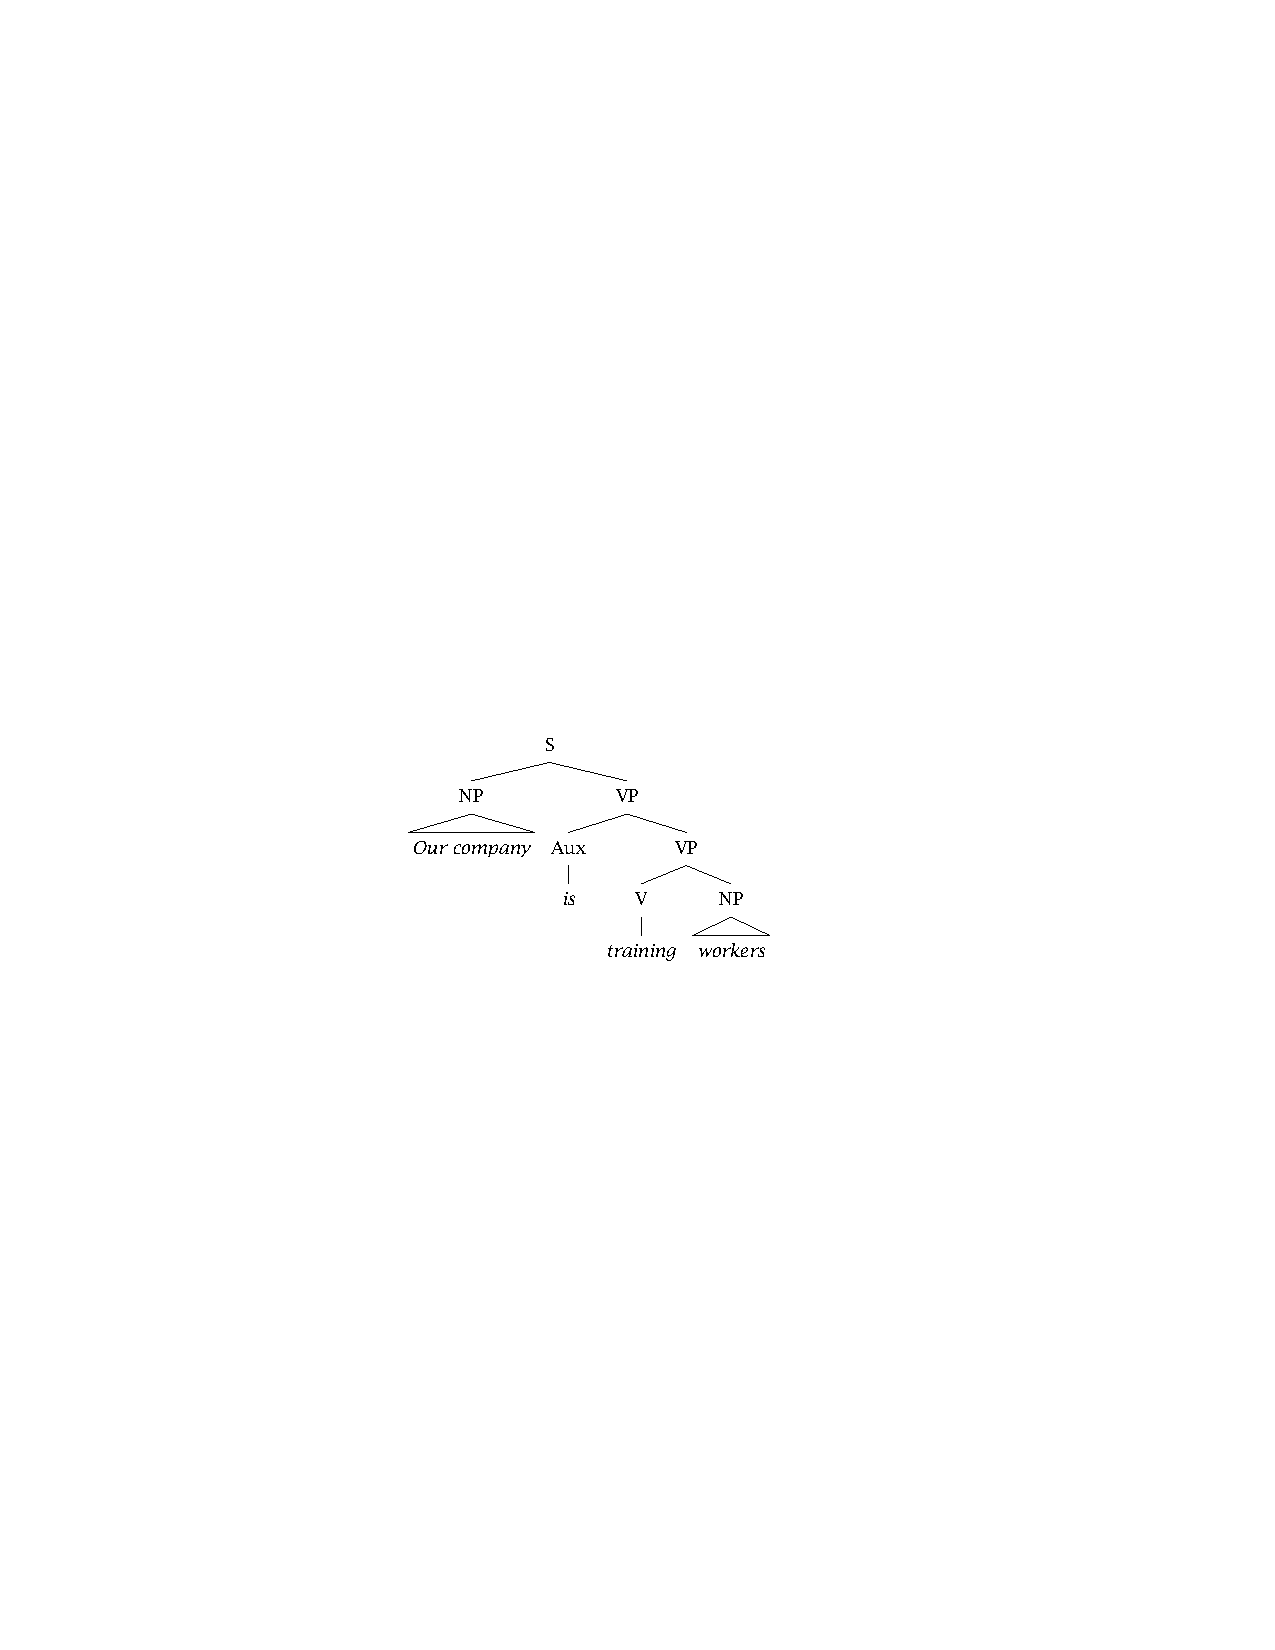
\includegraphics[width=0.5\textwidth]{figures/manning_parse.pdf}
    \caption{A parse of ``{\it Our company is training workers}''}
    \label{fig:manning_parse}
\end{figure}

The machine hears the sentence ``{\it Our company is training workers}'' and
infers the parse in Fig.~\ref{fig:manning_parse}. Then, we can make a simple set
of rules (again!) to let the machine answer questions about this sentence, kinds
of questions that imply that the machine has understood the sentence (language).
For instance, given a question ``{\it Who is training workers?}'', the machine
can answer by noticing that the question is asking for the subject of the verb
phrase
``{\it is training}'' acted on the object ``{\it workers}'' and that the subject
is ``{\it Our company}''.

\paragraph{Side Note: Bayesian Language Understanding} This generative view of
languages fits quite well with Bayesian modelling (see, e.g.,
\cite{perfors2006poverty}.) There exists a hidden mechanism, or a set of
generating rules and a rule governing their composition, which can be modelled
as a latent variable $Z$.  Given these rules, a language or a sentence $X$ is
generated according to the conditional distribution $P(X|Z)$. Then,
understanding language (by humans) is equivalent to computing the posterior
distribution over all possible sets of generating rules and their compositional
rules (i.e., $P(Z|X)$.) This answers the question of what is the most likely
mechanism underlying the observed language.

Furthermore, from the perspective of machines, Bayesian approach is attractive.
In this case, we assume to know {\it the} set of rules in advance and let the
latent variable $Z$ denote the specific configuration (use) of those rules.
Given this sequence of applying the rules, a sentence $X$ is generated via the
conditional distribution $P(X|Z)$. Machine understanding of language is
equivalent to inferring the posterior distribution over $Z$ given $X$.

For more details about Bayesian approaches (in the context of machine learning),
please, refer to \cite{bishop2006pattern} or take the course DS-GA 1005
Inference and Representation by Prof. David Sontag.

\paragraph{Understanding vs. Using} 
What's clear from this example is that in this generative view of languages,
there is a clear separation between understanding and using. Inferring the
generating rules from a given sentence is {\it understanding}, and answering a
question based on this understanding, {\it using}, is a separate activity.
Understanding part is done when the underlying (true) structure has been
determined regardless of how this understanding be used.

To put it in a slightly different wording, language understanding does not
require its use, or downstream tasks. In this road that we will {\em not} take
in this course, understanding exists as it is, regardless of what the understood
insight/knowledge will be used for. And, this is the reason why we do not walk
down this road.

\subsection{Road we {\it will} take}

\subsubsection{Language as a Function}

In this course, we will view a natural/human language as ``{\it a system
intended to communicate ideas from a speaker to a hearer}''
\cite{winograd1972understanding}. What this means is that we do not view a
language as a separate entity that exists on its own. Rather, we view a whole
system or behaviour of {\it communication} as a language. Furthermore, this view
dictates that we must take into account the world surrounding a speaker and a
hearer in order to understand language.

Under this view of language, language or rather its usage become somewhat
similar to action or behaviour. Speaking of something is equivalent to acting on
a listener, as both of them influence the listener in one way or another. The
purpose of language is then to influence another by efficiently communicate
one's will or intention.\footnote{
    Chomsky does not agree: ``{\it it is wrong to think of human use of language
    as characteristically informative, in fact or in intention.}''
    \cite{chomsky1968linguistic}.
} This hints at how language came to be (or may have come to be): (evolution)
language has evolved to facilitate the exchange of ideas among people (learning)
humans learn language by being either encouraged or punished for the use of
language. This latter view on how language came to be is similar in spirit to
the behaviourism of B. F. Skinner (``{\it necessary mediation of reinforcement by
another organism}'' \cite{skinner2014verbal}.)

This is a radical departure from the generative view of human language, where
language existed on its own and its understanding does not necessarily require
the existence of the outside world nor the existence of a listener. It is no
wonder why Chomsky was so harsh in criticizing Skinner's work in
\cite{chomsky1959review}. 
This departure, as I see it, is the departure toward a functional view of
language. {\it Language is a function of communication}. 

\subsubsection{Language Understanding as a Function Approximation}

Let's make a large jump here such that we consider this function as a
mathematical function.  This function (called language) takes as input the state
of the surrounding world, the speaker's speech, either written, spoken or signed
and the listener's mental state\footnote{
    We assume here that a such thing exists however it is represented in
    our brain.
} Inside the function, the listener's mental state is updated to incorporate the
new idea from the speaker's speech. The function then returns a response by the
listener (which may include ``no response'' as well) and a set of non-verbal
action sequences (what would be the action sequence if the speaker insulted
the listener?).

In this case, language understanding, both from humans' and machines'
perspective, boils down to figuring out the internal working of this function.
In other words, we understand language by learning the internal mechanism of the
function.  Furthermore, this view suggests that the underlying structures of
language are heavily dependent on the surrounding environment (context) as well
as on the target task. The former (context dependence) is quite clear, as the
function takes as input the context, but the latter may be confusing now.
Hopefully, this will become clearer later in the course.

How can we approximate this function? How can we figure out the internal working
mechanism of this function? What tools do we have?

\paragraph{Language Understanding by Machine Learning}
This functional view of languages suddenly makes machine learning a very
appealing tool for understanding human languages. After all, function
approximation is {\em the} core of machine learning. Classification is a
classical example of function approximation, clustering is a function
approximation where the target is not given, generative modeling learns a
function that returns a probability of an input, and so on.

When we approximate a function in machine learning, the prime ingredient is
data. We are given data which was either generated from this function
(unsupervised learning) or well fit this function (supervised learning), based
on which we adjust our approximation to the function, often iteratively, to best
fit the data. But, I must note here that it does not matter how well the approximated
function fits the data it was fitted to, but matters how well this approximation fits
{\em unseen} data.\footnote{
    This is a matter of generalization, and we will talk
    about this more throughout the course.
}

In language understanding, this means that we collect a large data set of input
and output pairs (or conversations together with the recording of the
surrounding environment) and fit some arbitrary function to well predict the
output given an input. We probably want to evaluate this approximation in a
novel conversation. If this function makes a conversation just like a person,
voil\`{a}, we made a machine that passed the Turing test.  Simple, right?

\paragraph{Problem}
Unfortunately, as soon as we try to do this, we run into a big problem. This
problem is not from machine learning nor languages, but the definition of this
function of language.

Properly approximating this function requires us to either simulate or record
the whole world (in fact, the whole universe.) For, this function takes as input
and maintains as internal state the surrounding world (context) and the mental
state of the individual (speaker.) This is unavoidable, if we wanted to very
well approximate this function as a whole.

It is unclear, however, whether we want to approximate the full function. For a
human to survive, yes, it is likely that the full function is needed. But, if
our goal is restricted to a certain task (such as translation, language
modelling, and so on), we may not want to approximate this function fully. We
probably want to approximate only a subset of this whole function. For instance,
if our goal is to understand the process of translation from one language to
another, we can perhaps ignore all but the speech input to the function and all
but the speech output from the function, because often a (trained) person can
translate a sentence in one language to another without knowing the whole
context.

This latter approach to language understanding--approximating a partial function
of languages-- will be at the core of this course. We will talk about various
language tasks that are a part of this whole function of language. These tasks
will include, but are not limited to, language modelling, machine translation,
image/video description generation and question answering. For these tasks and
potentially more, we will study how to use machine learning, or more
specifically deep learning, to solve these tasks by approximating sub-functions
of language.


\section{Function Approximation as Supervised Learning}

Throughout this course, we will extensively use artificial neural
networks\footnote{
    From here on, I will simply drop artificial and call them neural networks.
    Whenever I say ``neural network'', it refers to artificial neural networks.
}
to approximate (a part of) the function of natural language. This makes it
necessary for us to study the basics of neural networks first, and this lecture
and a couple of subsequent ones are designed to serve this purpose.

\subsection{Function Approximation: Parametric Approach}

\subsubsection{Expected Cost Function}

Let us start by defining a data distribution $p_{\text{data}}$.
$p_{\text{data}}$ is defined over a pair of input and output vectors, $\vx \in
\II^d$ and $\vy \in \OO^k$, respectively. $\II$ and $\OO$ are respectively sets
of all possible input and output values, such as $\RR$, $\left\{ 0, 1\right\}$
and $\left\{0, 1, \ldots, L\right\}$. This data distribution is not known to us.

The goal is to find a relationship between $\vx$ and $\vy$. More specifically,
we are interested in finding a function $f:\RR^d \to \OO^k$ that generates the
output $\vy$ given its corresponding input $\vx$. The very first thing we should
do is to put some constraints on the function $f$ to make our search for the
correct $f$ a bit less impossible. In this lecture, and throughout the course, I
will consider only a parametric function $f$, in which case the function is
fully specified with a set of parameters $\TT$.

Next, we must define a way to measure how well the function $f$ approximates the
underlying mechanism of generation ($\vx \to \vy$). Let's denote by $\hat{\vy}$ the 
output of the function with a particular set $\TT$ of parameters and a given input
$\vx$:
\begin{align*}
    \hat{\vy} = f_{\TT}(\vx)
\end{align*}
How well $f$ approximates the true generating function is equivalent to how far
$\hat{\vy}$ is from the correct output $\vy$. Let's use $D(\hat{\vy}, \vy)$ for
now call this distance\footnote{
    Note that we do not require this distance to satisfy the triangular
    inequality, meaning that it does not have to be a distance. However, I will
    just call it distance for now.
}
between $\hat{\vy}$ and $\vy$

It is clear that we want to find $\TT$ that minimizes $D(\hat{\vy}, \vy)$ for
every pair in the space ($RR^d \times \OO^k$). But, wait, every pair equally
likely? Probably not, for we do not care how well $f_{\TT}$ approximates the
true function, when a pair of input $\vx$ and output $\vy$ is unlikely, meaning
we do not care how bad the approximation is, if $p_\text{data}(\vx, \vy)$ is
small. However, this is a bit difficult to take into account, as we must decided
on the threshold below which we consider any pair irrelevant.

Hence, we {\em weight} the distance between the approximated $\hat{\vy}$ and the
correct $\vy$ of each pair $(\vx, \vy)$ in the space by its probability $p(\vx,
\vy)$. Mathematically saying, we want to find 
\begin{align*}
    \arg\min_{\TT} \int_{\vx} \int_{\vy} p_{\text{data}}(\vx, \vy) D(\hat{\vy}, \vy) \dd{\vx}
    \dd{\vy},
\end{align*}
where the integral $\int$ should be replaced with the summation $\sum$ if any of
$\vx$ and $\vy$ is discrete.

We call this quantity being minimized with respect to the parameters $\TT$ a
cost function $C(\TT)$. This is equivalent to computing the {\em expected}
distance between the predicted output $\hat{\vy}$ and the correct one $\vy$:
\begin{align}
    \label{eq:expected_cost}
    C(\TT) =& \int_{\vx} \int_{\vy} p_{\text{data}}(\vx, \vy) D(\hat{\vy}, \vy) \dd{\vx}
    \dd{\vy}, \\
    =& \E_{(\vx,\vy) \sim p_{\text{data}}}\left[ D(\hat{\vy}, \vy) \right] 
\end{align}
This is often called an expected loss or risk, and minimizing this cost function
is referred to as {\em expected risk minimization}~\cite{Vapnik1995}.

Unfortunately $C(\TT)$ cannot be (exactly) computed for a number of reasons. The
most important reason among them is simply that we don't know what the data
distribution $p_{\text{data}}$ is. Even if we have access to $p_{\text{data}}$,
we can exactly compute $C(\TT)$ only with heavy assumptions on both the data
distribution and the distance function.\footnote{Why?} 

\subsubsection{Empirical Cost Function}

This does not mean that we are doomed from the beginning. Instead of the
full-blown description of the data distribution $p_{\text{data}}$, we will
assume that someone miraculously gave us a finite set of pairs drawn from the
data distribution. We will call this a training set $D$:
\begin{align*}
    D=\left\{ (\vx^1, \vy^1), \ldots, (\vx^N, \vy^N) \right\}.  
\end{align*}

As we have access to the samples from the data distribution, we can use Monte
Carlo method to approximate the expected cost function $C(\TT)$ such that
\begin{align}
    \label{eq:empirical_cost}
    C(\TT) \approx \tilde{C}(\TT) = \frac{1}{N} \sum_{n=1}^N D(\hat{\vy^{n}},
    \vy^{n}).
\end{align}
We call this approximate $\tilde{C}(\TT)$ of the expected cost function, an
empirical cost function (or empirical risk or empirical loss.)

Because empirical cost function is readily computable, we will mainly work with
the empirical cost function not with the expected cost function. However, keep
in mind that at the end of the day, the goal is to find a set of parameters that
minimizes the {\em expected} cost.


\subsection{Learning as Optimization}

We often call this process of finding a good set of parameters that minimizes
the expected cost {\em learning}. This term is used from the perspective of a
machine which implements the function $f_{\TT}$, as it {\em learns} to
approximate the true generating function $f$ from training data.

From what I have described so far, it may have become clear even without me
mentioning that learning is {\em optimization}. We have a clearly defined
function (the empirical cost function $\tilde{C}$) which needs to be minimized
with respect to its input $\TT$.

\subsubsection{Gradient-based Local Iterative Optimization}
There are many optimization algorithms one can use to find a set of parameters
that minimizes $\tilde{C}$. Sometimes, you can even find the optimal set of
parameters in a closed form equation.\footnote{
    One such example is a linear regression where 
    \begin{itemize}
        \item $f_{\TT=\left\{ \mW\right\}}(\vx) = \mW \vx$
        \item $D(\hat{\vy}, \vy) = \frac{1}{2} \| \hat{\vy} - \vy \|^2$
    \end{itemize}
    In this case, the optimal $\mW$ is 
    \begin{align}
        \label{eq:opt_lin}
        \mW = \mY \mX^\top (\mX \mX^\top)^{-1},
    \end{align}
    where
    \begin{align*}
        \mX = \left[ \vx^1; \ldots ;\vx^N\right], \mY = \left[ \vy^1; \ldots ;\vy^N\right]. 
    \end{align*}

    Try it yourself! 
}
In most cases, because there is no known closed-form solution, it is typical to
use an iterative optimization algorithm (see \cite{Fletcher1987} for in-depth
discussion on optimization.) 

By an {\em iterative} optimization, I mean an algorithm which refines its
estimate of the optimal set of parameters little by little until the values of
the parameters converge to the optimal (expected) cost function. Also, it is
worthwhile to note that most iterative optimization algorithms are {\em local},
in the sense that they do not require us to evaluate the whole parameter space,
but only a small subset along the path from the starting point to the
convergence point.\footnote{
    There are {\em global} optimization algorithms, but they are out of scope
    for this course. See, for instance, \cite{Brochu2010} for one such algorithm
    called Bayesian optimization.
}

Here I will describe the simplest one among those local iterative optimization
algorithms, called gradient descent (GD) algorithm. As the name suggests, this
algorithm depends entirely on the gradient of the cost function.\footnote{
    From here on, I will use the cost function to refer to the {\em empirical}
    cost function.
} 

The gradient of a function $\nabla \tilde{C}$ is a vector whose direction points
to the direction of the greatest rate of increase in the function's value and
whose magnitude measures this rate. At each point $\TT_t$ in the parameter
space, the gradient of the cost function $\nabla \tilde{C}(\TT_t)$ is the {\em
opposite} direction toward which we want to move the parameters. See
Fig.~\ref{fig:grad} for graphical illustration.

\begin{figure}
    \centering
    \begin{minipage}{0.6\textwidth}
        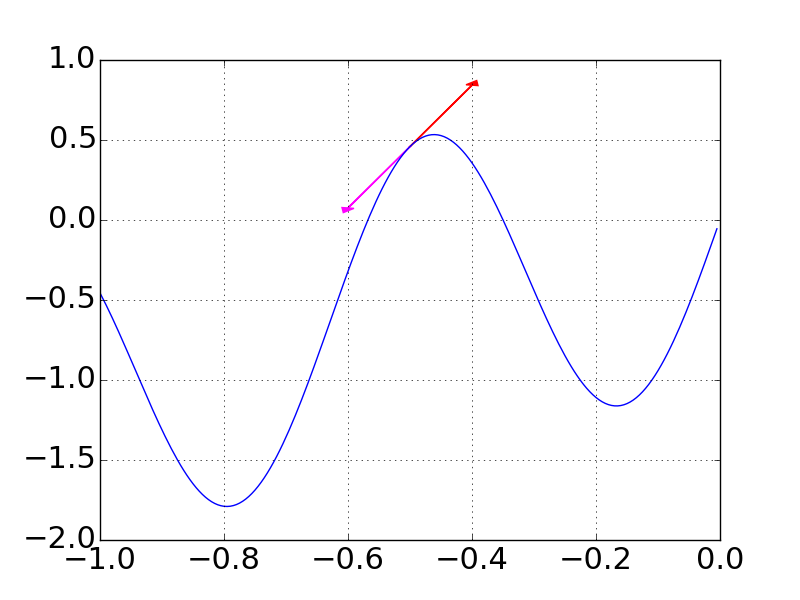
\includegraphics[width=\columnwidth]{figures/grad_figure.png}
    \end{minipage}
    \hfill
    \begin{minipage}{0.39\textwidth}
        \caption{(\textcolor{blue}{blue}) $f(x) = \sin(10 x) + x$.
            (\textcolor{red}{red}) a gradient at $x=-0.6$.
        (\textcolor{magenta}{magenta}) a negative gradient at $x=-0.6$.}
        \label{fig:grad}
    \end{minipage}
\end{figure}

One important point of GD that needs to be mentioned here is on how large a step
one takes each time. As clear from the magenta line (the direction opposite to
the direction given by the gradient) in Fig.~\ref{fig:grad}, if too large a step
is taken toward the negative gradient direction, the optimization process will
overshoot and miss the (local) minimum around $x=-0.8$. This step size, or
sometimes called learning rate, $\eta$ is one most important hyperparameter of
the GD algorithm.

Now we have all the ingredients for the GD algorithm: $\nabla \tilde{C}$ and
$\eta$. The GD algorithm iterates the following step:
\begin{align}
    \label{eq:GD}
    \TT \leftarrow \TT - \eta \nabla \tilde{C}(\TT).
\end{align}
The iteration continues until a certain stopping criterion is met, which we will
discuss shortly.

\subsubsection{Stochastic Gradient Descent}
This simple GD algorithm works surprisingly quite well, and it is a fundamental
basis upon which many advanced optimization algorithms have been built. I will
present a list of few of those advanced algorithms later on and discuss them
briefly. But, before going into those advanced algorithms, let's solve one tiny,
but significant issue of the GD algorithm.

This tiny, but significant issue arises especially often in machine learning.
That is, it is computationally very expensive to compute $\tilde{C}$ and
consequently its gradient $\nabla \tilde{C}$, thanks to the ever increasing size
of the training set $D$. 

Why is the growing size of the training set making it more and more
computationally demanding to compute $\tilde{C}$ and $\nabla \tilde{C}$?  This
is because both of them are essentially the sum of as many per-example costs as
there are examples in the training set. In other words,
\begin{align*}
    &\tilde{C}(\TT) = \frac{1}{N} \sum_{n=1}^N \tilde{C}(\vx^n, \vy^n | \TT), \\
    &\nabla \tilde{C}(\TT) = \frac{1}{N} \sum_{n=1}^N \nabla \tilde{C}(\vx^n, \vy^n | \TT).
\end{align*}
And, $N$ goes up to millions or billions very easily these days.

This enormous computational cost involved in each GD step has motivated the {\em
stochastic gradient descent} (SGD) algorithm~\cite{Robbins1951,Bottou1998}. 

First, recall from Eq.~\eqref{eq:empirical_cost} that the cost function we
minimize is the {\em empirical} cost function $\tilde{C}$ which is the
sample-based approximation to the {\em expected} cost function $C$. This
approximation was done by assuming that the training examples were drawn
randomly from the data distribution $p_{\text{data}}$:
\begin{align*}
    C(\TT) \approx \tilde{C}(\TT) = \frac{1}{N} \sum_{n=1}^N D(\hat{\vy^{n}},
    \vy^{n}).
\end{align*}
In fact, as long as this assumption on the training set holds, we can always
approximate the expected cost function with a fewer number of training examples:
\begin{align*}
    C(\TT) \approx \tilde{C}_\MM (\TT) = \frac{1}{|\MM|} \sum_{m \in \MM}
    D(\hat{\vy^{m}}, \vy^m),
\end{align*}
where $M \ll N$ and $\MM$ is the indices of the examples in this much smaller
subset of the training set. We call this small subset a {\em minibatch}.

Similarly, this leads to a minibatch-based estimate of the gradient as well:
\begin{align*}
    \nabla \tilde{C}_\MM (\TT) = \frac{1}{|\MM|} \sum_{m \in \MM} \nabla
    D(\hat{\vy^m}, \vy^m).
\end{align*}

It must now be clear to you where I am headed toward. At each GD step, instead
of using the full training set, we will use a small subset $\MM$ which is
randomly selected to compute the gradient estimate. In other words, we use
$\tilde{C}_\MM$ instead of $\tilde{C}$, and $\nabla \tilde{C}_\MM$ instead of
$\nabla \tilde{C}$, in Eq.~\eqref{eq:GD}. 

Because computing $\tilde{C}_\MM$ and $\nabla \tilde{C}_\MM$ is independent of
the size of the training set, we can use SGD to make as many steps as we want
without worrying about the growing size of training examples. This is highly
beneficial, as regardless of how many training examples you used to compute the
gradient, we can only take a tiny step toward that descending direction.
Furthermore, the increased level of noisy in the gradient estimate due to the
small sample size has been suspected to help reaching a better solution in 
high-dimensional non-convex problems (such as those in training deep neural
networks) \cite{Lecun1998a}.\footnote{
    Why would this be the case? It is worth thinking about this issue further.
}

We can set $M$ to be any constant, and in an extreme, we can set it to $1$ as
well. In this case, we call it online SGD.\footnote{
    Okay, this is not true in a strict sense. SGD is an online algorithm with
    $M=1$ originally, and using $M>1$, is a variant of SGD, often called,
    minibatch SGD. However, as using minibatches ($M>1$) is almost always the
    case in practice, I will refer to minibatch SGD as SGD, and to the original
    SGD as online SGD.
} Surprisingly, already in 1951, it was shown that using a single example each
time is enough for the SGD to converge to a minimum (under certain conditions,
obviously) \cite{Robbins1951}.

This SGD algorithm will be at the core of this course and will be discussed
further in the future lectures.


\subsection{When do we stop learning?}
\label{sec:model_selection}

From here on, I assume that we approximate the ground truth function by
iteratively refining its set of parameters, in most cases using {\em stochastic
gradient descent}. In other words, learning of a machine that approximates the
true generating function $f$ happens gradually as the machine goes over the
training examples little by little over time.

Let us go over again what kind of constraints/issue we have first:
\begin{enumerate}
    \item Lack of access to the expected cost function $C(\TT)$
    \item Computationally expensive empirical cost function $\tilde{C}(\TT)$
    \item (Potential) non-convexity of the empirical cost function
        $\tilde{C}(\TT)$
\end{enumerate}

The most severe issue is that we do not have access to the expected cost
function which is the one we want to minimize in order to work well with {\em
any} pair of input $\vx$ and output $\vy$. Instead, we have access to the
empirical cost function which is a finite sample approximation to the expected
cost function. 

\begin{figure}
    \centering
    \begin{minipage}{0.6\textwidth}
        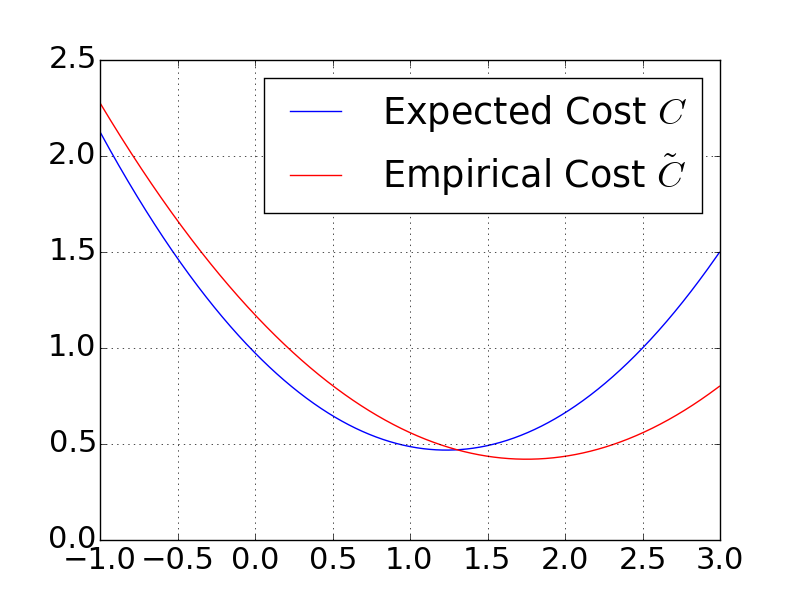
\includegraphics[width=\columnwidth]{figures/cost_figure.png}
    \end{minipage}
    \hfill
    \begin{minipage}{0.39\textwidth}
        \caption{(\textcolor{blue}{blue}) Expected cost function $C(\TT)$.
            (\textcolor{red}{red}) Empirical cost function $\tilde{C}(\TT)$.
            The underlying true generating function was $f(x) = \sin(10x) + x$.
            The cost function uses the squared Euclidean distance.
            The empirical cost function was computed based on 10 noisy
            examples of which $x$'s were sampled from the uniform distribution
        between $0$ and $1$. For each sample input $x$, noise from zero-mean Gaussian
    distribution with standard deviation $0.01$ was added to $f(x)$ to emulate
the noisy measurement channel.}
        \label{fig:cost}
    \end{minipage}
\end{figure}

Why is this a problem? Because, we do not have a guarantee that the (local)
minimum of the empirical cost function corresponds to the (local) minimum of the
expected cost function. An example of this mismatch between the expected and
empirical cost functions is shown in Fig.~\ref{fig:cost}.

As in the case shown in Fig.~\ref{fig:cost}, it is not desirable to minimize the
empirical cost function perfectly. The parameters that perfectly minimize the
empirical cost function (in the case of
Fig.~\ref{fig:cost}, the slope $a$ of a linear function $f(x) = a x$) will
likely be a sub-optimal cost for the expected cost function about which we
really care. 

\subsubsection{Early Stopping}
What should we do? There are many ways to avoid this weird contradiction where
we want to optimize the cost function well but not too well. Among those, one
most important trick is {\em early stopping}, which is only applicable when
iterative optimization is used.

First, we will split the training set $D$ into two partitions $D_{\train}$ and
$D_{\val}$.\footnote{
    Later on, we will split it further into three partitions.
}
We call them a training set and a validation set, respectively. In practice it
is a good idea to keep $D$ much larger than $D'$, because of the reasons that
will become clear shortly.

Further, let us define the training cost as
\begin{align}
    \label{eq:train_c}
    \tilde{C}(\TT) = C_{\train}(\TT) = \frac{1}{|D_{\train}|} \sum_{(x,y) \in
    D_{\train}} D_{\train}(\hat{y}, y),
\end{align}
and the validation cost as
\begin{align}
    \label{eq:val_c}
    C_{\val}(\TT) = \frac{1}{|D_{\val}|} \sum_{(x,y) \in D_{\val}} D(\hat{y}, y).
\end{align}
With these two cost functions we are all ready to use early stopping now. 

After every few updates using SGD (or GD), the validation cost function is
evaluated with the current set of parameters. The parameters are updated (i.e.,
the training cost function is optimized) until the validation cost does not
decrease, or starts to increase instead of decreasing.

That's it! It is almost free, as long as the size of the validation set is
reasonable, since each evaluation is at most as expensive as computing the
gradient of the empirical cost function. Because of the simplicity and
effectiveness, this early stopping strategy has become {\em de facto} standard
in deep learning and in general machine learning.

The question that needs to be asked here is what the validation cost function
does here. Clearly, it approximates the expected cost function $C$, similarly to
the empirical cost function $\tilde{C}$ as well as the training cost function
$C_{\train}$. In the infinite limit of the size of either training or validation
set, they should coincide, but in the case of a finite set, those two cost
functions differ by the noise in sampling (sampling pairs from the data
distribution) and observation (noise in $\vy=f(\vx)$.)

The fact that we explicitly optimize the training cost function implies that
there is a possibility (in fact, almost surely in practice) that the set of
parameters found by this optimization process may capture not only the
underlying generating function but also noise in the observation and sampling
procedure. This is an issue, because we want our machine to approximate the true
generating function not the noise process involved. 

The validation cost function measures both the true generating structure as well
as noise injected during sampling and observation. However, assuming that noise
is not correlated with the underlying generating function, noise introduced in
the validation cost function differs from that in the training cost function. In
other words, the set of parameters that perfectly minimizes the training cost
function (thereby capturing even noise in the training set) will be penalized
when measured by the validation cost function. 

\subsubsection{Model Selection}
In fact, the use of the validation cost does not stop at the early stopping.
Rather, it has a more general role in model selection. First, we must talk about
model selection itself.

This whole procedure of optimization, or learning, can be cast as a process of
searching for the best {\em hypothesis} over the entire space $\HH$ of
hypotheses.  Here, each hypothesis corresponds to each possible function (with a
unique set of parameters and a unique functional form) that takes the input
$\vx$ and output $\vy$. In the case of regression ($\vx \in \RR^d$ and $\vy \in
\RR$), the hypothesis space includes an $n$-th order polynomial function 
\begin{align*}
    f(x) = \sum_{\sum_{k=1}^d i_k = n, i_k \geq 0}
    a_{i_1,i_2,\ldots,i_k} \prod_{k'=1}^d x_{k'}^{i_k},
\end{align*}
where $a_{i_1,i_2,\ldots,i_k}$'s are the coefficients, and 
any other functional form that you can imagine as long as it can process $\vx$
and return a real-valued scalar.  In the case of neural networks, this space
includes all the possible model architectures which are defined by the number of
layers, the type of nonlinearities, the number of hidden units in each layer and
so on. 

Let us use
$M \in \HH$ to denote one hypothesis.\footnote{
    $M$, because each hypothesis corresponds to one learning {\em machine}.
} One important thing to remember is that the parameter space is only a subset
of the hypothesis space, because the parameter space is defined by a family of
hypotheses (the parameter space of a linear function cannot include a set of
parameters for a second-order polynomial function.)

Given a definition of expected cost function, we can {\em score} each hypothesis
$M$ by the corresponding cost $C_M$. Then, the whole goal of function
approximation boils down to the search for a hypothesis $M$ with the minimal
expected cost function $C$. But, of course, we do not have access to the
expected cost function and resort to the empirical cost function based on a
given training set. 

The optimization-based approach we discussed so far searches for the best
hypothesis based on the empirical cost iteratively. However, because of the
issue of {\em overfitting} which means that the optimization algorithm overshot
and missed the local minimum of the expected cost function (because it was aimed
at the local minimum of the empirical cost function), I introduced the concept
of early stopping based on the validation cost.

This is unfortunately not satisfactory, as we have only searched for the best
hypothesis inside a small subset of the whole hypothesis space $\HH$. What if
another subset of the hypothesis space includes a function that better suits the
underlying generating function $f$? Are we doomed?

It is clearly better to try more than one subsets of the hypothesis space. For
instance, for a regression task, we can try linear functions ($\HH_1$),
quadratic (second-order polynomial) functions ($\HH_2$) and sinusoidal functions
($\HH_3$). Let's say for each of these subsets, we found the best hypothesis
(using iterative optimization and early stopping); $M_{\HH_1}$, $M_{\HH_2}$ and
$M_{\HH_3}$. Then, the question is how we should choose one of those hypotheses.

Similar to what we've done with early stopping, we can use the validation cost
to compare these hypotheses. Among those three we choose one that has the
smallest validation cost $C_{\val}(M)$.

This is one way to do {\em model selection}, and we will talk about another way
to do this later.

\subsection{Evaluation}

But, wait, if this is an argument for using the validation cost to {\em early
stop} the optimization (or learning), one needs to notice something weird. What
is it?

Because we used the validation cost to stop the optimization, there is a chance
that the set of parameters we found is optimal for the validation set (whose
structure consists of both the true generating function and sampling/observation
noise), but not to the general data distribution. This means that we cannot tell
whether the function estimate $\hat{f}$ approximating the true generating
function $f$ is a good fit by simply early stopping based on the validation
cost.  Once the optimization is done, we need yet another metric to see how well
the learned function estimate $\hat{f}$ approximates $f$.

Therefore, we need to split the training set not into two partitions but into
{\em three} partitions. We call them a training set $D_{\train}$, a validation
set $D_{\val}$ and a test set $D_{\test}$. Consequently, we will have three cost
functions; a training cost function $C_{\train}$, a validation cost function
$C_{\val}$ and a test cost function $C_{\test}$, similarly to
Eqs.~\ref{eq:train_c}--\ref{eq:val_c}.

This test cost function is the one we use to compare different hypotheses, or
models, fairly. Any hypothesis that worked best in terms of the test cost is the
one that you choose.

\paragraph{Let's not Cheat}
One most important lesson here is that you {\em must never look at a test set}.
As soon as you take a peak at the test set, it will influence your choice in the
model structure as well as any other hyperparameters biasing toward a better
test cost. The best option is to never ever look at the test set until it is
absolutely needed (e.g., need to present your result.)

\subsection{Linear Regression for Non-Linear Functions}

Let us start with a simple linear function to approximate a true generating
function such that
\begin{align*}
    \hat{\vy} = f(\vx) = \mW^\top \vx, 
\end{align*}
where $\mW \in \RR^{d \times l}$ is the weight matrix. In this case, this weight
matrix is the only parameter, i.e., $\TT=\left\{ \mW \right\}$.

The empirical cost function is then
\begin{align*}
    \tilde{C}(\TT) = \frac{1}{N} \sum_{n=1}^N \frac{1}{2} \left\| \vy^n - \mW^\top \vx^n
    \right\|^2_2.
\end{align*}

The gradient of the empirical cost function is
\begin{align}
    \label{eq:grad_lin}
    \nabla \tilde{C}(\TT) = -\frac{1}{N} \sum_{n=1}^N 
    \left( \vy^n - \mW^\top \vx^n\right)^\top \vx^n.
\end{align}

With these two well defined, we can use the iterative optimization algorithm,
such as GD or SGD, to find the best $\mW$ that minimizes the empirical cost
function.\footnote{
    In fact, looking at Eq.~\eqref{eq:grad_lin}, it's quite clear that you can
    compute the optimal $\mW$ analytically. See Eq.~\eqref{eq:opt_lin}.
}
Or, better is to use a validation set to stop the optimization
algorithm at the point of the minimal validation cost function (remember early
stopping?)

Now, but we are not too satisfied with a linear network, are we?

\subsubsection{Feature Extraction}
\label{sec:feature_extraction}

Why are we not satisfied?

First, we are not sure whether the true generating function $f$ was a linear
function. If it is not, can we expect linear regression to approximate the true
function well? Of course, not. We will talk about this shortly.

Second, because we were {\em given} $\vx$ (meaning we did not have much control
over what we want to measure as $\vx$), it is unclear how well $\vx$ represents
the input. For instance, consider doing a sales forecast of air conditioner at
one store which opened five years ago. The input $x$ is the number of days since
the opening date of the store (1 Jan 2009), and the output $y$ is the number of
units sold on each day.

Clearly, in this example, the relationship between $x$ and $y$ is not linear.
Furthermore, perhaps the most important feature for predicting the sales of air
conditioners is missing from the input $x$, which is a month (or a season, if
you prefer.) It is likely that the sales bottoms out during the winter (perhaps
sometime around December, January and February,) and it hits the peak during
summer months (around May, June and July.) In other words, if we look at how far
the month is away from July, we can predict the sales quite well even with 
linear regression.

Let us call this quantity $\phi(x)$, or equivalent {\em feature}, such that
\begin{align}
    \label{eq:feat_month}
    \phi(x) = \left| m(x) - \alpha \right|,
\end{align}
where $m(x) \in \left\{ 1,2,\ldots,12\right\}$ is the month of $x$ and
$\alpha=5.5$.  With this
feature, we can fit linear regression to better approximate the sales figure of
air conditioners. Furthermore, we can add yet another feature to improve the
predictive performance. For instance, one such feature can be which day of week
$x$ is. 

This whole process of extracting a good set of features that will make our
choice of parametric function family (such as linear regression in this case) is
called {\em feature extraction}. This feature extraction is an important step in
machine learning and has often been at the core of many applications such as
computer vision (the representative example is SIFT~\cite{lowe1999object}.)

Feature extraction often requires heavy knowledge of the domain in which this
function approximation is applied. To use linear regression for computer vision,
it is a good idea to use computer vision knowledge to extract a good set of
features. If we want to use it for environmental problems, we must first notice
which features must be important and how they should be represented for linear
regression to work. 

This is okay for a machine learning practitioner in a particular field, because
the person has in-depth knowledge about the field. There are however many cases
where there's simply not enough domain knowledge to exploit. To make the matter
worse, it is likely that the domain knowledge is not correct, making the whole
business of using manually extracted features futile.

\section{Neural Networks and Backpropagation Algorithm}

\subsection{Conditional Distribution Approximation}

I have mainly described so far as if the function we approximate or the function
we use to approximate returns only a constant value, as in one point $\vy$ in
the output space. This is however not true, and in fact, the function can return
anything including a {\em
distribution}~\cite{Bridle1990,denker1991transforming,bishop1994mixture}.

Let's first decompose the data distribution $p_{\data}$ into the product
of two terms:
\begin{align*}
    p_{\data}(\vx, \vy) = p_{\data}(\vx) p_{\data}(\vy |\vx).
\end{align*}
It becomes clear that one way to sample from $p_{\data}$ is to sample an input
$\vx^n$ from $p_{\data}(\vx)$ and subsequently sample the corresponding output
$\vy^n$ from the conditional distribution $p_{\data}(\vy | \vx^n)$. 

This implies that the function approximation of the generating function ($f:
\vx \to \vy$) is effectively equivalent to approximating the conditional
distribution $p_{\data}(\vy | \vx)$. This may suddenly sound much more
complicated, but it should not alarm you at all.  As long as we choose to use a
distribution parametrized by a small number of parameters to approximate the
conditional distribution $p_{\data}(\vy | \vx)$, this is quite manageable
without almost any modification to the expected and empirical cost functions we
have discussed. 

Let us use $\TT(\vx)$ to denote a set of parameters for the probability
distribution $\tilde{p}(\vy|\vx, \TT(\vx))$ approximating the true, underlying
probability distribution $p_{\data}(\vy|\vx)$. As the notation suggests, the
function now returns {\em the parameters of the distribution} $\TT(\vx)$ given
the input $\vx$. 

For example, let's say $\vy \in \left\{ 0, 1\right\}^k$ is a binary vector and
we chose to use independent Bernoulli distribution to approximate the
conditional distribution $p_{\data}(\vy | \vx)$. In this case, the parameters
that define the conditional distribution are the means of $k$ dimensions:
\begin{align}
    \label{eq:bernoulli}
    \tilde{p}(\vy | \vx) = \prod_{k'=1}^k p(y_{k'}|\vx) = 
    \prod_{k'=1}^k \mu_{k'}^{y_{k'}} (1-\mu_{k'})^{1-y_{k'}}.
\end{align}
Then the function $\TT(\vx)$ should output a $k$-dimensional vector of which
each element is between 0 and 1.

Another example: let's say $\vy \in \RR^k$ is a real-valued vector. It is quite
natural to use a Gaussian distribution with a diagonal covariance matrix to
approximate the conditional distribution $p(\vy | \vx)$:
\begin{align}
    \label{eq:gaussian}
    \tilde{p}(\vy | \vx) = \prod_{k'=1}^k \frac{1}{\sqrt{2\pi}\sigma_{k'}} 
\exp\left( \frac{(y_{k'} - \mu_{k'})^2}{2\sigma_{k'}^2} \right).
\end{align}
The parameters for this conditional distribution are $\TT(\vx) = \left\{ 
    \mu_1, \mu_2, \ldots, \mu_k, \sigma_1, \sigma_2, \ldots, \sigma_k
\right\}$, where $\mu_k \in \RR$ and $\sigma_k \in \RR_{>0}$.

In this case of probability approximation, it is natural to use
Kullback-Leibler (KL) divergence to measure the distance.\footnote{
    Again, we use a loose definition of the distance where triangular inequality
    is not enforced.
} 
The KL divergence from one distribution $P$ to the other $Q$ is
defined\footnote{
    Why don't I say the KL divergence between two distributions here? Because,
    the KL divergence is not a symmetric measure, i.e., $\KL(P\|Q) \neq
    \KL(Q\|P)$.
}
by
\begin{align*}
    \KL(P\|Q) = \int P(\vx) \log \frac{P(\vx)}{Q(\vx)} \dd{\vx}.
\end{align*}
In our case of function/distribution approximation, we want to minimize the KL
divergence from the data distribution $p_{\data}(\vy|\vx)$ to the approximate
distribution $\tilde{p}(\vy | \vx)$ averaged over the data distribution
$p_{\data}(\vx)$:
\begin{align*}
    C(\TT) = \int p_{\data}(\vx) \KL(p_{\data}\|\tilde{p}) \dd{\vx} = 
    \int p_{\data}(\vx) \int p_{\data}(\vy|\vx) \log \frac{p_{\data}
    (\vy|\vx)}{\tilde{p}(\vy|\vx)} \dd{\vy} \dd{\vx}.
\end{align*}
But again we do not have access to $p_{\data}$ and cannot compute this expected
cost function.

Similarly to how we defined the empirical cost function earlier, we must
approximate this expected KL divergence using the training set: 
\begin{align}
    \label{eq:kl_train}
    \tilde{C}(\TT) = \frac{1}{N} \sum_{n=1}^N -\log \tilde{p}(\vy^n|\vx^n).
\end{align}
As an example, if we choose to return the binary vector $\vy$ as in
Eq.~\eqref{eq:bernoulli}, the empirical cost function will be
\begin{align*}
    \tilde{C}(\TT) = -\frac{1}{N} \sum_{n=1}^N 
    \sum_{k'=1}^k y_{k'} \log \mu_{k'} + (1-y_{k'}) \log (1 - \mu_{k'}),
\end{align*}
which is often called a {\em cross entropy cost}. In the case of
Eq.~\eqref{eq:gaussian}, 
\begin{align}
    \label{eq:kl_gaussian}
    \tilde{C}(\TT) = -\frac{1}{N} \sum_{n=1}^N 
    \sum_{k'=1}^k \frac{(y_{k'} - \mu_{k'})^2}{2\sigma_{k'}^2} - \log
        \sigma_{k'}.
\end{align}

Do you see something interesting in Eq.~\eqref{eq:kl_gaussian}? If we assume
that the function outputs $1$ for all $\sigma_{k'}$'s, we see that this cost
function reduces to that using the Euclidean distance between the true output
$\vy$ and the mean $\vmu$. What does this mean?

There will be many occasions later on to discuss more about this perspective
when we discuss language modelling. However, one thing we must keep in our mind
is that there is nothing different between approximating a function and a
distribution.

\subsubsection{Why do we want to do this?}

Before we move on to the main topic of today's lecture, let's try to understand
why we want to output the distribution. Unlike returning a single point in the
space, the distribution returned by the function $f$ incorporates both the most
likely outcome $\hat{y}$ as well as the uncertainty associated with this value.

In the case of the Gaussian output in Eq.~\eqref{eq:gaussian}, the standard
deviation $\sigma_{k'}$, or the variance $\sigma_{k'}^2$, indicates how
uncertain the function is about the output centered at $\mu_{k'}$. Similarly,
the mean $\mu_{k'}$ of the Bernoulli output in Eq.~\eqref{eq:bernoulli} is
directly proportional to the function's confidence in predicting that the
$k'$-th dimension of the output is $1$.

\begin{figure}[ht]
    \centering
    \begin{minipage}{0.6\textwidth}
        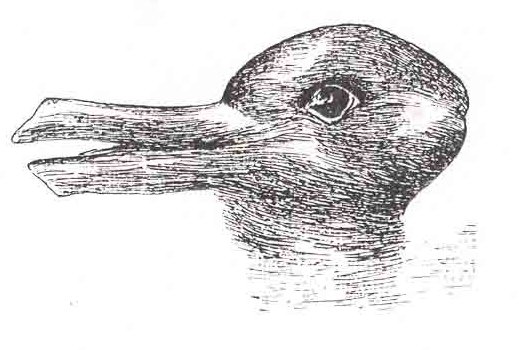
\includegraphics[width=\columnwidth]{figures/duck_rabbit.png}
    \end{minipage}
    \hfill
    \begin{minipage}{0.39\textwidth}
        \caption{Is this a duck or a rabbit? \cite{kuhn2012structure} At the end
        of the day, we want our function $f$ to return a conditional
    distribution saying that $p(\text{duck}|\vx) = p(\text{rabbit}|\vx)$,
instead of returning {\em the} answer out of these two possible answers.}
        \label{fig:duck_rabbit}
    \end{minipage}
\end{figure}

This is useful in many aspects, but one important aspect is that it reflects the
natural uncertainty of the underlying generating function. One input $\vx$ may
be interpreted in more than one ways, leading to two possible outputs, which
happens more often than not in the real world. For instance, the famous picture
in Fig.~\ref{fig:duck_rabbit} can be viewed as a picture of a duck or a picture
of a rabbit, in which case the function needs to output the probability
distribution by which the same probability mass is assigned to both a duck and a
rabbit. Furthermore, there is observational noise that cannot easily be
identified and ignored by the function, in which case the function should return
the uncertainty due to the observational noise along with the most likely (or
the average) prediction.

\subsubsection{Other Distributions}

I have described two distributions (densities) that are widely used: 
\begin{itemize}
    \itemsep 0em
    \item Bernoulli distribution: binary classification
    \item Gaussian distribution: real value regression
\end{itemize}
Here, let me present one more distribution which we will use almost everyday
through this course.

\paragraph{Categorical Distribution: Multi-Class Classification}

Multi-class classification is a task in which each example belongs to one of $K$
classes. For each input $x$, the problem reduces to find a probability $p_k(x)$
of the $k$-th class under the constraint that 
\begin{align*}
    \sum_{k=1}^K p_k(x)=1
\end{align*}

It is clear that in this case, the function $f$ returns $K$ values $\left\{
\mu_1, \mu_2, \ldots, \mu_K \right\}$, each of which is between $0$ and $1$.
Furthermore, the sum of $\mu_k$'s must sum to $1$. This can be achieved easily
by letting $f$ to compute affine transformation of $x$ (or $\phi(x)$) to return
$K$ (unbounded) real values followed by a so called {\em softmax}
function~\cite{Bridle1990}:
\begin{align*}
    \mu_k = \frac{\exp(w_k^\top \phi(x) + b_k)}{\sum_{k'=1}^K \exp(w_{k'}^\top
    \phi(x) + b_k)},
\end{align*}
where $w_k \in \RR^{\dim(\phi(x))}$ and $b_k \in \RR$ are the parameters of
affine transformation.

In this case, the (empirical) cost function based on the KL divergence is
\begin{align*}
    C(\TT) = \frac{1}{N} \sum_{n=1}^N \sum_{k=1}^K \II_{k=y^n} \mu_k,
\end{align*}
where 
\begin{align*}
    \II_{k=y^n} = \left\{ 
        \begin{array}{c c}
            1, & \text{if }k=y^n \\
            0, & \text{otherwise}
        \end{array}
        \right.
\end{align*}

\subsection{Feature Extraction is also a Function}

We talked about the manual feature extraction in the previous lecture (see
Sec.~\ref{sec:feature_extraction}. But, this is quite unsatisfactory, because
this whole process of manual feature extraction is heavily dependent on the
domain knowledge, meaning that we cannot have a generic principle on which we
design features. This raises a question: instead of manually designing features
ourselves, is it possible for this to happen automatically?

One thing we notice is that the feature extraction process $\phi(\vx)$ is
nothing but a {\em function}. A function of a function is a function, right? In
other words, we will extend our definition of the function to include the
feature extraction function:
\begin{align*}
    \hat{\vy} = f(\phi(\vx)).
\end{align*}

We will assume that the feature extraction function $\phi$ is also parametrized,
and its parameters are included in the set of parameters which includes those of
$f$. As an example, $\alpha$ in Eq.~\eqref{eq:feat_month} is a parameter of the
feature extraction $\phi$.

A natural next question is which family of parametric functions we should use
for $\phi$. We run into the same issue we talked about earlier in
Sec.~\ref{sec:model_selection}: the size of hypothesis space is simply too
large!

Instead of choosing one great feature extraction function, we can go for a stack
of simple transformations which are all learned.\footnote{
    A great article about this was posted recently in
    \url{http://colah.github.io/posts/2014-03-NN-Manifolds-Topology/}.
}
Each transformation can be as simple as affine transformation followed by a
simple point-wise nonlinearity:
\begin{align}
    \label{eq:layer}
    \phi_0(\vx) = g(\mW_0 \vx + \vb_0),
\end{align}
where $\mW_0$ is the weight matrix, $\vb_0$ is the bias and $g$ is a point-wise
nonlinearity such as $\tanh$.\footnote{
    Some of the widely used nonlinearities are
    \begin{itemize}
        \item Sigmoid: $\sigma(x) = \frac{1}{1+\exp(-x)}$
        \item Hyperbolic function: $\tanh(x) = \frac{1-\exp(-2x)}{1+\exp(-2x)}$
        \item Rectified linear unit: $\rect(x) = \max(0, x)$
    \end{itemize}
}

One interesting thing is that if the dimensionality of the transformed feature
vector $\phi_0(\vx)$ is {\em much} larger than that of $\vx$, the function
$f(\phi_0(\vx))$ can approximate any function from $\vx$ to $\vy$ under some
assumptions, even when the parameters $\mW_0$ and $\vb_0$ are randomly
selected!~\cite{Cover1965} 

The problem solved, right? We just put a huge matrix $\mW_0$, apply some
nonlinear function $g$ to it and fit linear regression as I described earlier.
We don't even need to touch $\mW_0$ and $\vb_0$. All we need to do is replace
the input $\vx^n$ of all the pairs in the training set to $\phi_0(\vx^n)$.

In fact, there is a group of researchers claiming to have figured this out by
themselves less than a decade ago (as of 2015) who call this model an {\em
extreme learning machine}~\cite{Huang2006}. There have been some debates about
this so-called extreme learning machine. Here I will not make any comment
myself, but would be a good exercise for you to figure out why there has been
debates about this.

But, regardlessly, this is not what we want.\footnote{
    And, more importantly, I will not accept any final project proposal whose
    main model is based on the ELM.
}
What we want is to fully tune the whole thing.

\subsection{Multilayer Perceptron}

The basic idea of multilayer perceptron is to stack a large number of those
feature extraction {\em layers} in Eq.~\eqref{eq:layer} between the input and
the output. This idea is as old as the whole field of neural network research,
dating back to early 1960s~\cite{Rosenblatt1962}. However, it took many more
years for people to figure out a way to tune the whole network, both $f$ and
$\phi$'s together. See \cite{schmidhuber2015deep} and \cite{lecun2015deep}, if you
are interested in the history.

\subsubsection{Example: Binary classification with a single hidden unit}

Let us start with the simplest example. The input $x \in \RR$ is a real-valued
scalar, and the output $y \in \left\{0,1\right\}$ is a binary value
corresponding to the input's label. The feature extractor $\phi$ is defined as
\begin{align}
    \label{eq:phi}
    \phi(x) = \sigma(u x + c),
\end{align}
where $u$ and $c$ are the parameters. The function $f$ returns the mean of the
Bernoulli conditional distribution $p(y|x)$:
\begin{align}
    \label{eq:f}
    \mu = f(x) = \sigma(w \phi(x) + b).
\end{align}
In both of these equations, $\sigma$ is a sigmoid function:
\begin{align*}
    \sigma(x) = \frac{1}{1+\exp(-x)}.
\end{align*}

We use the KL divergence to measure the distance between the true conditional
distribution $p(y|x)$ and the predicted conditional distribution $\hat{p}(y|x)$.
\begin{align*}
    \KL(p\|\hat{p}) =& \sum_{y \in \left\{0, 1\right\}} p(y|x) \log
    \frac{p(y|x)}{\hat{p}(y|x)} \\
    =& \sum_{y \in \left\{0, 1\right\}} p(y|x) \log p(y|x) - p(y|x) \log
    {\hat{p}(y|x)}.
\end{align*}
Note that the first term in the summation $p(y|x) \log p(y|x)$ can be safely
ignored in our case. Why? Because, this does not concern $\tilde{p}$ which is
one we change in order to minimize this KL divergence.

Let's approximate this KL divergence with a single sample from $p(y|x)$ and
leave only the relevant part. We will call this a per-sample cost:
\begin{align}
    \label{eq:cost_bernoulli}
    C_x =& - \log \hat{p}(y|x) \\
    =& - \log \mu^y (1-\mu)^{1-y} \\
    =& - y \log \mu - (1-y) \log (1-\mu),
\end{align}
where $\mu$ is from Eq.~\eqref{eq:f}.  It is okay to work with this per-sample
cost function instead of the full cost function, because the full cost function
is almost always the (unweighted) sum of these per-sample cost functions. See
Eq.~\eqref{eq:empirical_cost}.

We now need to compute the gradient of this cost function $C_x$ with respect to
all the parameters $w$, $b$, $u$ and $c$. First, let's start with $w$:
\begin{align*}
    \frac{\partial C_x}{\partial w} = \frac{\partial C_x}{\partial \mu}
    \frac{\partial \mu}{\partial \underline{\mu}}
    \frac{\partial \underline{\mu}}{\partial w},
\end{align*}
which is a simple application of chain rule of derivatives. Compare this to
\begin{align*}
    \frac{\partial C_x}{\partial b} = \frac{\partial C_x}{\partial \mu}
    \frac{\partial \mu}{\partial \underline{\mu}}
    \frac{\partial \underline{\mu}}{\partial b}.
\end{align*}
In both equations, $\underline{\mu} = w \phi(x) + b$ which is the input to $f$.


Both of these derivatives {\em share} $\frac{\partial C_x}{\partial
\mu}\frac{\partial \mu}{\partial \underline{\mu}}$, where
\begin{align}
    \label{eq:out_deriv}
    \frac{\partial C_x}{\partial \mu} \underbrace{\frac{\partial \mu}{\partial
    \underline{\mu}}}_{=\mu'} = 
    -\frac{y}{\mu}\mu' +
    \frac{1-y}{1-\mu}\mu' 
    = \frac{-y + y\mu + \mu - y\mu }{\mu(1-\mu)}\mu' 
    = \frac{\mu - y}{\mu(1-\mu)}\mu' 
    = \mu - y,
\end{align}
because the derivative of the sigmoid function $\frac{\partial \mu}{\partial
\underline{\mu}}$ is
\begin{align*}
    \mu' = \mu (1-\mu).
\end{align*}
Note that this corresponds to computing the difference between the correct label
$y$ and the predicted label (probability) $\mu$.

Given this output derivative $\frac{\partial C_x}{\partial \underline{\mu}}$, all we need to
compute are
\begin{align*}
    &\frac{\partial \underline{\mu}}{\partial w} = \phi(x) \\
    &\frac{\partial \underline{\mu}}{\partial b} = 1.
\end{align*}
From these computations, we see that
\begin{align}
    \label{eq:c_w}
    &\frac{\partial C_x}{\partial w} = (\mu - y) \phi(x), \\
    \label{eq:c_b}
    &\frac{\partial C_x}{\partial b} = (\mu - y).
\end{align}

Let us continue on to $u$ and $c$. We can again rewrite the derivatives w.r.t.
these into
\begin{align*}
    \frac{\partial C_x}{\partial u} =& \frac{\partial C_x}{\partial
    \underline{\mu}}
    \frac{\partial \underline{\mu}}{\partial \phi}
    \frac{\partial \phi}{\partial \underline{\phi}}
    \frac{\partial \underline{\phi}}{\partial u} \\
    \frac{\partial C_x}{\partial c} =& \frac{\partial C_x}{\partial
    \underline{\mu}}
    \frac{\partial \underline{\mu}}{\partial \phi}
    \frac{\partial \phi}{\partial \underline{\phi}}
    \frac{\partial \underline{\phi}}{\partial c},
\end{align*}
where $\underline{\phi}$ is the input to $\phi$ similarly to $\underline{\mu}$
was to the input to $\mu$.

There are two things to notice here. First, we already have $\frac{\partial
C_x}{\partial \underline{\mu}}$ from computing the derivatives w.r.t. $w$ and
$b$, meaning there is no need to re-compute it. Second, $\frac{\partial
\underline{\mu}}{\partial \underline{\phi}}$ is shared between the derivatives
w.r.t. $u$ and $c$.

Therefore, we first compute $\frac{\partial \underline{\mu}}{\partial
\underline{\phi}}$:
\begin{align*}
    \frac{\partial \underline{\mu}}{\partial \phi}\underbrace{\frac{\partial \phi}{\partial
    \underline{\phi}}}_{=\phi'} = w \phi' = w \phi(x) (1- \phi(x))
\end{align*}
Next, we compute 
\begin{align*}
    &\frac{\partial \underline{\phi}}{\partial u} = x \\
    &\frac{\partial \underline{\phi}}{\partial c} = 1.
\end{align*}

Now all the ingredients are there:
\begin{align*}
    \frac{\partial C_x}{\partial u} =& (\mu -y) w \phi(x) (1-\phi(x)) x \\
    \frac{\partial C_x}{\partial c} =& (\mu -y) w \phi(x) (1-\phi(x)).
\end{align*}

The most important lession to learn from here is that most of the computations
needed to get the derivatives in this seemingly complicated multilayered
computational graph (multilayer perceptron) are {\em shared}. At the end of the
day, the amount of computation needed to compute the gradient of the cost
function w.r.t. all the parameters in the network is only as expensive as
computing the cost function itself.

\subsubsection{Example: Binary classification with more than one hidden units}
\label{sec:example2}

Let us try to generalize this simple, or rather simplest model, into a slightly
more general setting. We will still look at the binary classification but with
multiple hidden units and a multidimensional input such that:
\begin{align*}
    \phi(x) = U x + c,
\end{align*}
where $U \in \RR^{l \times d}$ and $c \in \RR^l$. Consequently, $w$ will be a
$l$-dimensional vector.

The output derivative $\frac{\partial C_x}{\partial \mu}\frac{\partial
\mu}{\partial \underline{\mu}}$ stays same as before. See
Eq.~\eqref{eq:out_deriv}.
However, we note that the derivative of $\underline{\mu}$ with respect to $w$
should now differ, because it's a vector.\footnote{
    The Matrix Cookbook \cite{petersen2008matrix} is a good reference for this
    section.
}
Let's look at what this means.

The $\underline{\mu}$ can be expressed as
\begin{align}
    \label{eq:mu_vec}
    \underline{\mu} = w^\top \phi(x) + b = \sum_{i=1}^l w_i \phi_i(x) + b.
\end{align}
In this case, we can start computing the derivative with respect to each element
of $w_i$ separately:
\begin{align*}
    \frac{\partial \underline{\mu}}{\partial w_i} = \phi_i(x),
\end{align*}
and will put them into a vector:
\begin{align*}
    \frac{\partial \underline{\mu}}{\partial w} = \left[ 
        \frac{\partial \underline{\mu}}{\partial w_1}, \frac{\partial
        \underline{\mu}}{\partial w_2}, \ldots, \frac{\partial
        \underline{\mu}}{\partial w_l}
    \right]^\top = \left[ \phi_1(x), \phi_2(x), \ldots, \phi_l(x) \right]^\top
    = \phi(x)
\end{align*}

Then, the derivative of the cost function $C_y$ with respect to $w$ can be
written as
\begin{align*}
    \frac{\partial C_y}{\partial w} = (\mu -y) \phi(x),
\end{align*}
in which case nothing really changed from the case of a single hidden unit in
Eq.~\eqref{eq:c_w}.

Now, let's look at $\frac{\partial C_y}{\partial \phi}$. Again, because
$\phi(x)$ is now a vector, there has to be some changes. Because $\frac{\partial
C_y}{\partial \underline{\mu}}$ is already computed, we only need to look at
$\frac{\partial \underline{\mu}}{\partial \phi}$. In fact, the procedure for
computing this is identical to that for computing $\frac{\partial
\underline{\mu}}{\partial w}$ due to the symmetry in Eq.~\eqref{eq:mu_vec}. That
is,
\begin{align*}
    \frac{\partial \underline{\mu}}{\partial \phi} = w
\end{align*}

Next, what about $\frac{\partial \phi}{\partial \underline{\phi}}$? Because the
nonlinear activation function $\sigma$ is applied element-wise, we can simply
compute this derivative for each element in $\phi(x)$ such that
\begin{align*}
    \frac{\partial \phi}{\partial \underline{\phi}} = 
    \diag\left(\left[ \phi_1'(x), \phi_2'(x), \ldots, \phi_l'(x)
    \right]^\top\right),
\end{align*}
where $\diag$ returns a diagonal matrix of the input vector. In short, we will
denote this as $\phi'$

Overall so far, we have got
\begin{align*}
    \frac{\partial C_y}{\partial \underline{\phi}} = 
    (\mu - y)w^\top \phi'(x) = (\mu - y) (w \odot \diag(\phi'(x))),
\end{align*}
where $\odot$ is an element-wise multiplication.

Now it is time to compute $\frac{\partial
\underline{\phi}}{\partial U}$:
\begin{align*}
    \frac{\partial \underline{\phi}}{\partial U} = \frac{\partial U^\top
    x}{\partial U} = x,
\end{align*}
according to the Matrix Cookbook \cite{petersen2008matrix}. Then, let's look at
the whole derivative w.r.t. $U$:
\begin{align*}
    \frac{\partial C_y}{\partial U} = (\mu - y) (w \odot \diag(\phi'(x)))
    x^\top.
\end{align*}
Note that all the vectors in this lecture note are {\em column} vectors.

For $c$, it's straightforward, since 
\begin{align*}
    \frac{\partial \underline{\phi}}{\partial c} = 1.
\end{align*}


\subsubsection{Automating Backpropagation}

This procedure, presented as two examples, is called a {\em backpropagation}
algorithm. If you read textbooks on neural networks, you see a fancier way to
explain this backpropagation algorithm by introducing a lot of fancy terms such
as {\em local error} $\delta$ and so on. But, personally I find it much easier
to understand backpropagation as a clever application of the chain rule of
derivatives to a directed acyclic graph (DAG) in which each node computes a certain
function $\phi$ using the output of the previous nodes. I will refer to this
DAG as a computational graph from here on.

\begin{figure}[ht]
    \centering
    \begin{minipage}{0.48\textwidth}
        \centering
        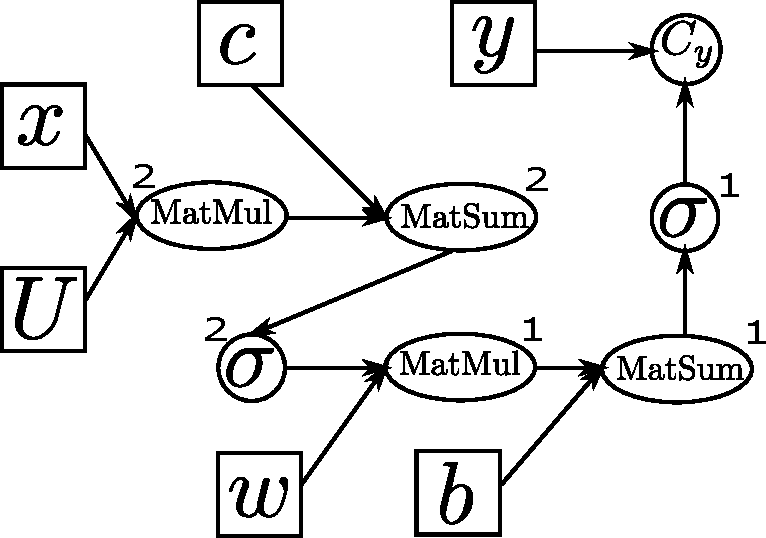
\includegraphics[width=0.9\textwidth]{figures/comp_graph.pdf}
    \end{minipage}
    \hfill
    \begin{minipage}{0.48\textwidth}
        \centering
        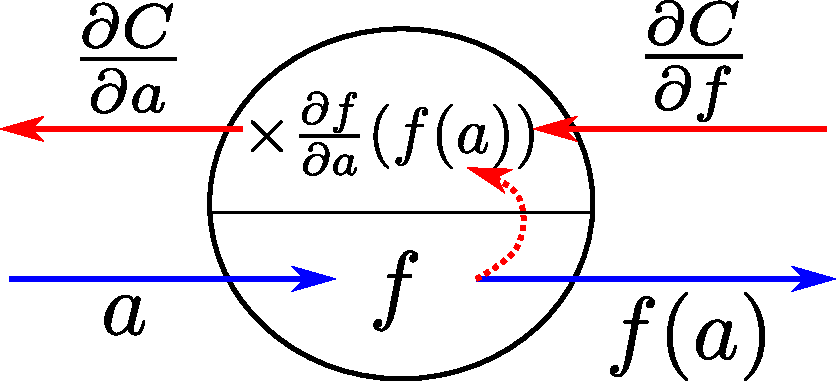
\includegraphics[width=0.9\textwidth]{figures/comp_node.pdf}
    \end{minipage}

    \begin{minipage}{0.48\textwidth}
        \centering
        (a)
    \end{minipage}
    \hfill
    \begin{minipage}{0.48\textwidth}
        \centering
        (b)
    \end{minipage}
    \caption{(a) A graphical representation of the computational graph of the
    example network from Sec.~\ref{sec:example2}. (b) A graphical illustration
    of a function node ({\color{blue} $\to$}: forward pass, {\color{red}
$\leftarrow$}: backward pass.)}
    \label{fig:comp_graph}
\end{figure}

A typical computational graph looks like the one in Fig.~\ref{fig:comp_graph}~(a).
This computational graph has two types of nodes; (1) function node ($\bigcirc$)
and (2) variable node ($\Box$). There are four different types of function
nodes; (1) $\text{MatMul}(A,B) = AB$, (2) $\text{MatSum}(A,B)=A+B$, (3)
$\sigma$: element-wise sigmoid function  and (4) $C_y$: cost node. The variables
nodes correspond to either parameters or data ($x$ and $y$.) Each function node
has a number associated with it to distinguish between the nodes of the same
function.

Now, in this computational graph, let us start computing the gradient using the
backpropagation algorithm. We start from the last code, $C_y$, by computing
$\frac{\partial C_y}{\partial y}$ and $\frac{\partial C_y}{\partial \sigma^1}$.
Then, the function node $\sigma^1$ will compute its own derivative
$\frac{\partial \sigma^1}{\partial \text{MatSum}^1}$ and multiply it with
$\frac{\partial C_y}{\partial \sigma^1}$ passed {\em back} from the function
node $C_y$. So far we've computed
\begin{align}
    \label{eq:dC_dMS1}
    \frac{\partial C_y}{\partial \text{MatSum}^1} = \frac{\partial C_y}{\partial \sigma^1} \frac{\partial \sigma^1}{\partial
    \text{MatSum}^1}
\end{align}

The function node MatSum$^1$ has two inputs $b$ and the output of MatMul$^1$.
Thus, this node computes two derivatives $\frac{\partial
\text{MatSum}^1}{\partial b}$ and $\frac{\partial \text{MatSum}^1}{\partial
\text{MatMul}^1}$. Each of these is multiplied with the backpropagated
derivative $\frac{\partial C_y}{\partial \text{MatSum}^1}$ from
Eq.~\eqref{eq:dC_dMS1}. At this point, we already have the derivative of the
cost function $C_y$ w.r.t. one of the parameters $b$:
\begin{align*}
    \frac{\partial C_y}{\partial b} = \frac{\partial C_y}{\partial
    \text{MatSum}^1} \frac{\partial \text{MatSum}^1}{\partial b}
\end{align*}

This process continues mechanically until the very beginning of the graph (a set
of root variable nodes) is reached. All we need in this process of
backpropagating the derivatives is that each function node implements both {\em
forward computation} as well as {\em backward computation}. In the backward
computation, the function node received the derivative from the next function
node, evaluates its own derivative with respect to the inputs (at the point of
the forward activation) and passes theses
derivatives to the corresponding previous nodes. See
Fig.~\ref{fig:comp_graph}~(b) for the graphical illustration.

Importantly, the inner mechanism of a function node does not change depending on
its context (or equivalently where the node is placed in a computational graph.)
In other words, if each type of function nodes is implemented in advance, it
becomes trivial to build a complicated neural network (including multilayer
perceptrons) and compute the gradient of the cost function (which is one such
function node in the graph) with respect to all the parameters as well as all
the inputs.

This is a special case, called the reverse mode, of automatic
differentiation.\footnote{
    If anyone's interested in digging more into the whole field of automatic
    differentiation, try to Google it and you'll find tons of materials.
} It is probably the most valuable tool in deep learning, and fortunately many
widely used toolkits such as Theano~\cite{bergstra2010theano,bastien2012theano}
have implemented this reverse mode of automatic differentiation with an
extensive number of function nodes used in deep learning everyday.

Before finishing this discussion on automating backpropagation, I'd like you to
think of pushing this even further. For instance, you can think of each function
node returning not its numerical derivative on its backward pass, but a
computational sub-graph computing its derivative. This means that it will return
a {\em computational graph of gradient}, where the output is the derivatives of
all the variable nodes (or a subset of them.) Then, we can use the same facility
to compute the second-order derivatives, right? 

\subsubsection{What if a Function is {\em not} Differentiable?}

From the description so far, one thing we notice is that backpropagation works
only when each and every function node (in a computational graph) is
differentiable. In other words, the nonlinear activation function must be chosen
such that almost everywhere it is differentiable. All three activation functions
I have presented so far have this property.

\paragraph{Logistic Functions}
A sigmoid function is defined as
\begin{align*}
    \sigma(x) = \frac{1}{1+\exp(-x)},
\end{align*}
and its derivative is
\begin{align*}
    \sigma'(x) = \sigma(x) (1 - \sigma(x)).
\end{align*}

A hyperbolic tangent function is
\begin{align*}
    \tanh(x) =  \frac{\exp(2x) -1}{\exp(2x) + 1},
\end{align*}
and its derivative is 
\begin{align*}
    \tanh'(x) = \left(\frac{2}{\exp(x)+\exp(-x)}\right)^2.
\end{align*}

\paragraph{Piece-wise Linear Functions}

I described a rectified linear unit (rectifier or ReLU,
\cite{nair2010rectified,glorot2011deep}) earlier:
\begin{align*}
    \rect(x) = \max(0, x).
\end{align*}
It is clear that this function is not strictly differentiable, because of the
discontinuity at $x=0$. However, the chance of the input to this rectifier lands
exactly at $0$ has zero probability, meaning that we can forget about this
extremely unlikely event. The derivative of the rectifier in this case is
\begin{align*}
    \rect'(x) = \left\{ 
        \begin{array}{l l}
            1, & \text{if }x > 0 \\
            0, & \text{if }x \leq 0
        \end{array}
        \right.
\end{align*}

Although the rectifier has become the most widely used nonlinearity, especially,
in deep learning's applications to computer vision,\footnote{
    Almost all the winning entries in ImageNet Large Scale Visual Recognition
    Challenges (ILSVRC) use a convolutional neural network with rectifiers. See
    \url{http://image-net.org/challenges/LSVRC/}.
}
there is a small issue with the rectifier. That is, for a half of the input
space, the derivative is zero, meaning that the error (the output derivative
from Eq.~\eqref{eq:out_deriv}) will be not well propagated through the rectifier
function node.

In \cite{goodfellow2013maxout}, the rectifier was extended to a maxout unit so
as to avoid this issue of the existence of zero-derivative region in the input
to the rectifier. The maxout unit of rank $k$ is defined as
\begin{align*}
    \maxout(x_1, \ldots, x_k) = \max(x_1, \ldots, x_k),
\end{align*}
and its derivative as
\begin{align*}
    \frac{\partial \maxout}{\partial x_i}(x_1, \dots, x_k) = 
    \left\{
        \begin{array}{l l}
            1, & \text{if } \max(x_1, \ldots, x_k) = x_i \\
            0, & \text{otherwise}
        \end{array}
        \right.
\end{align*}
This means that the derivative is backpropagated only through one of the $k$
inputs.

\paragraph{Stochastic Variables}
These activation functions work well with the backpropagation algorithm, because
they are differentiable almost everywhere in the input space. However, what
happens if a function is non-differentiable at all. One such example is a binary
stochastic node, which is computed by
\begin{enumerate}
    \itemsep 0em
    \item Compute $p = \sigma(x)$, where $x$ is the input to the function node.
    \item Consider $p$ as a mean of a Bernoulli distribution, i.e., $\BB(p)$.
    \item Generate one sample $s \in \left\{ 0, 1\right\}$ from the Bernoulli distribution.
    \item Output $s$.
\end{enumerate}
Clearly there is no derivative of this function node. 

Does it mean that we're doomed in this case? Fortunately, no. Although I will
not discuss about this any further in this course,
Bengio~et~al.~\cite{bengio2013estimating} provide an extensive list of
approaches we can take in order to compute the derivative of the stochastic
function nodes.



\section{Recurrent Neural Networks and Gated Recurrent Units}




\alert{\it Soon to appear}


















%\subsection{Why Deep Neural Networks?}
%
%\alert{TBD}
%
%
%\subsection{History of Neural Network Architecture}
%
%It is quite controversial when deep learning, or in general neural network
%research, began and how it has evolved over
%years~\cite{schmidhuber2015deep,lecun2015deep}.\footnote{
%    Also, see ``Critique of Paper by "Deep Learning Conspiracy" (Nature 521 p
%    436)'' by Schmidhuber: 
%    \url{https://plus.google.com/100849856540000067209/posts/9BDtGwCDL7D}.
%}
%Aside all these controversies, I will say that 
%
%
%\subsection{Linear Regression to Multilayer Perceptron}
%
%\alert{TBD}
%
%\subsection{Learning as Optimization}

























\nocite{pesetsky1999linguistic}




\bibliographystyle{abbrv}
\bibliography{lecture_note}


\end{document}






